\chapter{Background}
\label{chap:background}
This chapter will cover the basic background of rowing, the sports science which guides rowing training, and how an athletes body responds to training stimulus. Next, a review of performance modelling will explore the development of human performance modelling since the introduction of the basic Bannister model in 1975 \autocite{Bannister1976}. The section will outline how training load and performance can be quantified, and explain the way these approximations are used in various performance models to date.

\section{A brief Introduction to Rowing}
Rowing is an Olympic sport, raced across a 2,000 metre course, typically lasting six to seven minutes. It is classed as a power-endurance sport, this means training is focused on building aerobic, anerobic, and power while also developing rowing technique \autocite{Mäestu2005}. Most time is spent building endurance, next most time is spent building anerobic capacity, finally building strength and power through strength and condition sessions \autocite{Seiler2006}. The importance of power is more significant in rowing than in cycling given the relatively short duration of exertions, with longer distance racing typically only covering five to seven kilometers, or fifteen to twenty-five minutes. Conversely, road cycling, tends to last for a longer period of time, where the shortest races might last two hours. There are many different approaches to how training is conducted and which energy systems are targeted for improvements in efficiency or strength. This section will discuss the basic training principles which guide training, the way athletes respond to different kinds of training loads, and how performance is evaulated in rowing.

\subsection{\label{sub:training_principles}Training Principles}
Generally when a coach builds a training plan they have a few factors they can work with: volume, the amount of mileage or total time spent training, sessions intensity, how hard the given session is meant to be, and finally the frequency, or the time spent in different intensity zones. There are various ways to measure intensity, including heart rate, blood lactate concentration, velocity at maximal oxygen uptake (VO2 max), and relative perceived exertion (RPE) \autocite{Rosenblat2019}. 

\subsubsection{Training zones}
Rowers tend to use heart rate zones or blood lactate concentration depending on access to the equipment to test blood lacate. Typically when a rower uses calculated aerobic zones each zone will be a percentage of \maxHR. Following this approach, zones are defined as follows:
\begin{description}
  \item[Z1] "Very Light" intensity, 50\% - 60\% of \maxHR
  \item[Z2] "Light" intensity, 60\%-70\% of \maxHR
  \item[Z3] "Moderate" intensity, 70\%-80\% of \maxHR
  \item[Z4] "Hard" intensity, 80\%-90\% of \maxHR
  \item[Z5] "Maximum" intensity, 90\%-100\% of \maxHR
\end{description}
The exact definition of these zones varies in the literature, as does the method to calculate \maxHR without a specific test. However, most high level athletes will have completed some kind of stress test to determine their \maxHR in order to train more effectively on their prescribed zones.
A rower who uses lactate based training zones might use the following zones:
\begin{description}
  \item[T1]  basic oxygen utilization training (UT2) [lactate~=~0-2 mmol/L]
  \item[T2]  oxygen utilization training (UT1) [lactate~=~2-3.5 mmol/L]
  \item[T3]  anaerobic threshold training (AT) [lactate~=~3.5-4.5 mmol/L]
  \item[T4]  oxygen transport training (TR) [lactate~=~4.5-6 mmol/L]
  \item[T5]  anaerobic capacity training (AN) [lactate $\geq$ 6 mmol/L] \autocite{Das2022}
\end{description}
Depending on how rigorous the testing protocol was, Heart Rate zones may be calculated for each zone, these may vary from the aerobic zones calculated from \maxHR.

The most basic zone approximation approach uses three zones based around certain physiological thresholds, like, lacate thresholds ($\textnormal{LT}_\text{1}$ and $\textnormal{LT}_\text{2}$) and ventilatory thresholds. Cyclists may use critical power to determine these three basic zones, although this practice has not become popular in rowing training. The zones become simply, low-intensity, moderate-intensity, and high-intensity. 

\subsubsection{Blood lactate - A brief description}
Lactate is constantly produced by the body during the day. The concentration of blood lactate, measured in millimoles per litre (mmol/L), does not increase until the rate of lactate production surpasses the rate of lactate removal. Many things can affect the rate of lactate removal, training can improve the rate of lactate removal, with certain sessions targetting that adaptation. Blood lactate acts a biomarker used regularly to determine muscular fatigue during exercise. During a exercise lactate test a lactate profile is generated. Figure \ref{fig:lactateGraph} shows a chart showing two lactate profiles generated during two lactate tests about 14 weeks apart (98 days) in January and May of 2023. The test conducted saw the rower complete seven, four minute, efforts, at prescribed wattage targets. Details of each set of intervals can be found in \ref{sec:app-lactate-results}.
\begin{figure}
  \centering
  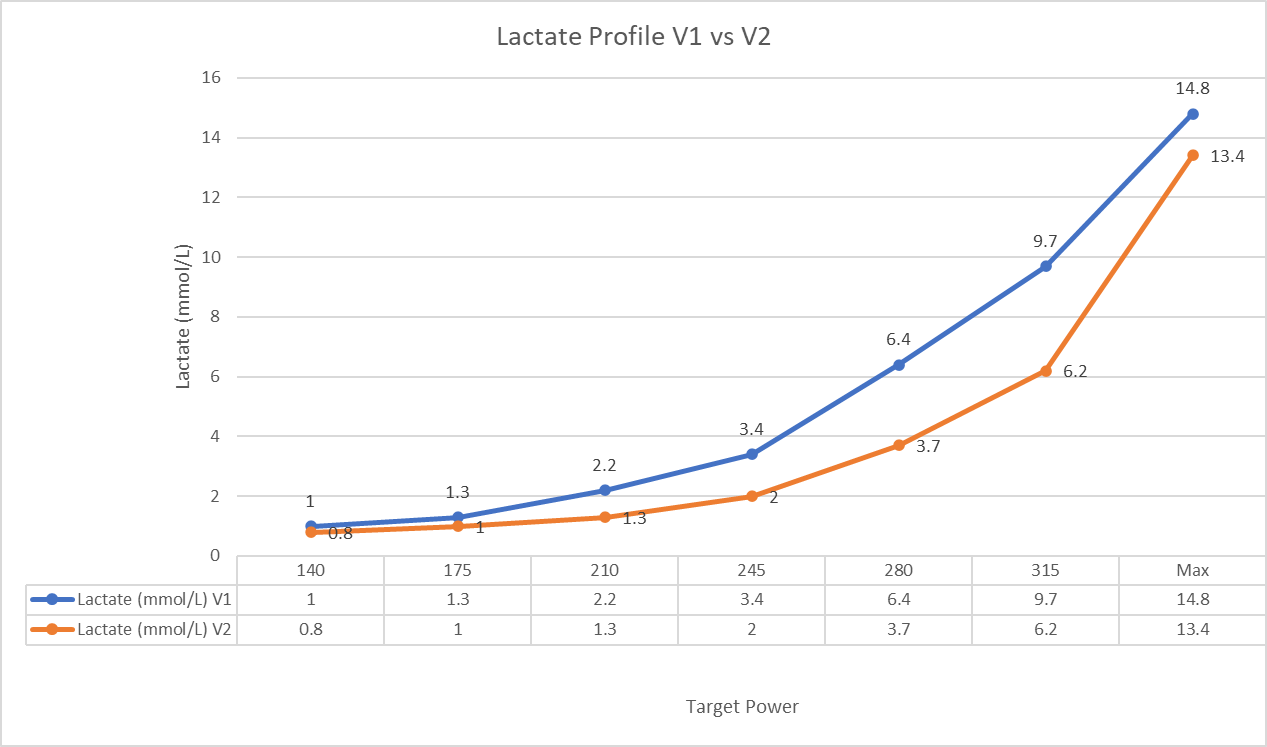
\includegraphics[width=\linewidth]{figures/lactateGraph.png}
  \caption[Lactate Profiles from January and May 2023]{Two lactate profiles completed 98 days apart following the protocol described above. Test one completed January 24, 2023. Test Two completed May 2, 2023}
  \label{fig:lactateGraph}
\end{figure}
These curves can be used to prescribe training as is described above.

\subsubsection{Training prescription and distribution}
There are a few different approaches for distributing intensity for endurance training. The three main methods are: polarised training, sweet spot or threshold training, and pyramidal training. This guides the final factor a coach considers when building a general training plan, frequency. For the purposes of comparing polarized training (POL), threshold training (THR), and pyramidal training (PYR), the more basic three zones of intensity will be used. The breakdown per zone for each training method is as follows:
\begin{description}
  \item[Polarised Training] Far more time spent in the low-intensity zone \autocite{Seiler2004}.

  \begin{description}
    \item[Low-Intensity] 75\%-85\% of total training volume
    \item[Medium-Intensity] 5\%-10\% of total training volume
    \item[High-Intensity] 5\%-10\% of total training volume  
  \end{description} 
  \item[Threshold Training] More time spent in the medium-intensity zone \autocite{Seiler2004}.

  \begin{description}
    \item[Low-Intensity] 45\%-55\% of total training volume
    \item[Medium-Intensity] 35\%-55\% of total training volume
    \item[High-Intensity] 15\%-20\% of total training volume  
  \end{description}
  \item[Pyramidal Training] Most time spent in low-intensity zone with progressively less time spent in higher zones \autocite{Selles2019}.

  \begin{description}
    \item[Low-Intensity] 75\%-85\% of total training volume
    \item[Medium-Intensity] 15\%-20\% of total training volume
    \item[High-Intensity] 5\%-10\% of total training volume  
  \end{description}
\end{description}

This report will not compare the effectiveness of different training distributions. Different distributions tend to be used by different sports, or depending on which energy system is being targeted. The use of polarized training is most common in rowing \autocite{Rosenblat2019}, although other training approaches have been used, especially around competition time.


\subsection{Energy Systems}
\label{sub:energy_systems}
In the human body there are two major types of skeletal muscle fibres, fast twitch, and slow twitch. Slow twitch muscles are used for longer, slower contractions where relative strength is low. Conversely, fast twitch muscles are shorter, faster contractions where strength is relatively higher. These types of fibres store energy differently and respond to training differently. Slow twitch muscles can be adapted to longer, lower effort, sessions and become resistant to fatigue, while fast twitch muscles fatigue easily, due to their lower glycogen capacity. Slow twitch muscle fibres have a low anaerobic capacity, while fast twitch muscle fibres have high anerobic capacities. These two kinds of fibres draw on two different energy systems: anaerobic and aerobic systems. These systems provide muscles with Adenosine Triphosphate (ATP) which is used by the mitochondria in the muscle fibre cells to produce energy, allowing the muscles to contract \cite{Göktepe2007}. 

The anaerobic system is used to provide energy to muscles to produce power without the use of oxygen. The anaerobic system typically provides energy for shorter periods of time. An immediate energy system can provide energy for 1-2 seconds of maximal work, this is typically used for resistance based strength training. More commonly in rowers, the short term energy system is used to provide energy to muscle fibres under significant strain. However, each time the energy system produces (ATP), lactate is also produced. This system is limited by an athletes ability to flush lactate from muscles. If the muscles are unable to flush the lactate quickly enough, the muscles will fatigue until failure forcing a stop to exercise. 

The aerobic, or long term energy, system is the slowest at providing energy to muscles. This system uses sugars, fats and oxygen to produce ATP. This system only works when large amounts of oxygen are available, which for rowers is typically during lower intensity sessions. Longer "steady state" sessions rely on the aerobic to provide energy to muscles, with these sessions also being used to build the aerobic system. By spending time in the appropriate training zones the aerobic system builds efficiency by creating new capillaries to support the slow twich fibres.

Rowers develop both their anaerobic and aerobic systems. Much of the winter season (typically September-March) is spent building the aerobic system, this is due to the longer length of any races done during this period, and to build a larger base on which to build a strong anerobic system. As the sprint racing season begins, or shortly before, more anerobic sessions will be introduced to build the system. Rowers will build their lactate tolerance, and spend more time at just-below-maximal efforts to prepare for the shorter race format.

% \subsection{Physiological Response to Training}
% Different people respond to training differently, for example, two people may be taking up a similar volume of oxygen (even $\textnormal{VO}_2$ utilization), but their muscles may be responding differently, producing different performances, or being able to sustain that load for different length of time. Differences in lactate threshold (LT), for example, can model the physiological state of an athlete during these efforts \autocite{Baldwin2000}. The goal for each training session is to, as efficiently as possible, become "fitter", in order to perform better. \textcite{Seiler2011} (2011) explored the effect of the use of different training intensities and durations on trained cyclists. 4x8min interval sessions yielded the most "\textit{pain for the gain}". Given that 

\subsection{Training Considerations}
When building a training plan many things are considered. Plans are typically built in macro-, meso-, and micro-cycles \cite{periodisation}. The macro-cycle in rowing will normally work on a yearly basis, with the overall target of performing at championship event at the end of the training year. 

Meso-cycles are typically seasonal or monthly cycles. For example, the autumn season is focused on building base fitness and forming a squad's technical style, there may be small races which a squad may attend, but any specific preparation for these events is unlikely. The winter months will be focussed on building the aerobic base, with some race preparation towards the end of the season being introduced. The spring season will see the first race events. Typically these are "Head races", longer races (5-6km) allowing the longer length, lower inensity sessions from the winter to be leveraged. This season will also an increase in interval and sprint race preparation in anticipation of the summer months. The summer season is the primary racing season, with the macro-cycle peak in performance. This meso-cycle will see a reduction in lower intensity aerobic sessions and an increase in anerobic intensity work to build fast-twitch muscle performances and the necessary racing performances of the shorter events.

Within these meso-cycles, there are micro-cycles typically lasting 7-14 days. It is crucial that these cycles are "periodised" appropriately. Periodisation is the budgeting of load across micro-cycles, ensuring athletes are experiencing the appropriate increase in intensity, followed by an appropriate length recovery period.

A coach will develop a training plan at the start of a new year, with a general idea of each cycle, and make adjustments as necessary throughout the year. If a coach had access to a system which could model the individual training responses for each athlete, individualised plans could be generated for each athlete, allowing the entire squad to train, and perform, at their physiological maximum. 

\subsubsection{Overtraining and burnout}
Training for endurance sports puts a large amount of strain physically, and mentally on athletes. Endurance athletes are conditioned to consistently push their bodies, making it difficult to identify when overtraining has occurred. Spending too much time in hard training zones without providing enough time to rest and recover leads to overtraining. Overtraining can be diagnosed when a performance decrease, as a result of training fatigued, has not gone away within two weeks of relative rest \cite{kayser2004chronic}. Overtraining can manifest symptoms physically and emotionally. Athletes may become depressed, chronically fatigued, and lose their appetites before a drop in performance. Ensuring training plans are appropriately periodised (load is managed in sustainable cycles of intensity and rest), and with enough variety in sessions to avoid monotony can help avoid overtraining. Athlete stress management outside of training is also crucial to managing overtraining.

Overtraining can often lead to burnout. Burnout is when an athlete gives up a sport entirely. With many athletes attaching their self-esteem to success in their sport, they risk burning out. This is particularly problematic when an athlete may be suffering from overtraining, or underperformance \cite{gustafsson2007burnout}.

Managing both overtraining and burnout are important when training, and can be considered when building a model of performance. Recognising overtraining can potentially prevent a promising athlete from retiring from their sport. By developing individual performance models, it can be easier to recognise overtraining and adjustments can be made to help the athlete recover more quickly.

\subsubsection{Tapering}
The concept of a taper is common among endurance athletes. Training blocks tend to be quite exhausting and typically leave athletes in an "over-reaching" state, they are constantly in a fatigued state. This encourages physiological adaptations but also negatively impacts performance. A taper period sees an athlete reduce their training load ahead of a competition \cite{Lawton2023}. Timing of the taper is important as athletes want to strike a balance between losing too much training time, and consequently fitness, and not having a long enough taper, and therfore still experiencing some training induced fatigue. Different taper strategies can be used, but typically session volume decreases, rather than session count. Typically as part of a taper a very short period (2-3 days) of high-intensity, interval, sessions is completed. This is followed by a longer period of recovery, or relative rest, in order to induce a "super-compensation" effect. This effect is a result of the body continuing to recover beyond the original baseline of fitness in anticipation of another period of high-intensity interval sessions. This results in a minor performance boost \cite{Kanwetz2016}.


\subsection{Performance}
There are two primary ways to measure a performance in rowing. First, on the rowing machine, a 2,000 meter, 6,000 meter, or 30 minute at stroke rate 20 (30 r20) test is normally used, depending on when during the season the test is done. This can be used to determine a rower's fitness and can be used to track progress for an athlete. These sessions are typically maximum effort sessions with some degree of taper (typically 4-7 days maximum) to elicit a peak performance. On the water, times can also be used to judge an entire crew, with external factors like wind direction and intensity, current flow, and temperature considered. Some boats and squads may use on the water telemetry to quantify the impact and power output of each rower. On-the-water performances may not always be peak efforts depending on a squad's seasonal focus or an event's progression (e.g. a maximal effort will rarely make an appearance in the heat stage of a heat-semi-final progression). Ergometer scores tend to be considered the purest way of quantifying a rower's performance, however, a combination of approaches can be used to quantify on-the-water performance.

\subsection{Summary}
Rowing training is quite time consuming for athletes. Many rowers will learn much of what has been discussed in this section to make better decisions themselves, or understand why training is done in a given way. The focus for a majority of the training cycle is to build a strong aerobic base in order to allow for higher "peak", ideally coinciding with the peak event for a season of training. For international athletes this will be a yearly cycle targetting World Championships, which is part of a four-yearly cycle targetting the Olympics. For national level athletes, national championships are typically the target, with Henley Royal Regatta featuring as a season's target. Coaches will normally take into account season targets and rower proficiency and base fitness when generating training plans. The target of this project is to make it easier for coaches and more accessible for athletes who may be more independent. 

\section{A Review of Performance Modelling}
The first wide spread approach to modelling performance was developed by \textcite{Bannister1976} with the Banister Fitness - Fatigue model, and further refined by \textcite{Morton1990} when defining training impulse to determine fitness and fatigue. The use of machine learning, specifically artificial neural networks has since been introduced in approaches to model performance. In preparation for the 2000 Olympics in Sydney, \textcite{Edelmannnusser2002} successfully predicted Olympic performances within an error of 0.05 seconds across a total time of 2:12.64 (min:sec) for the 200m backstroke event. \textcite{Edelmannnusser2002} specifically consider the limitation of using a linear model, such as the model proposed by \textcite{Bannister1976}, on training adaptation and performance; adaptation to training is inherently a complex non-linear process. 

This section will review basic approaches to systems modelling, exploring metrics which are commonly used to guide models and some non-linear systems models which have been explored. 

\subsection{Quantifying Training Load (Fatigue)}
\subsubsection{Rate of perceived exertion (RPE)} \label{subsub:rpe}
Rate of perceived exertion (RPE) is a scale, originally introduced by Gunnar Borg, to measure an athlete's effort. The original scale ranged from 6-20, where 6 would be no exertion at all, and 20 is maximal effort. This scale ranges from 6-20 to correspond more easily with heart rate, as the scale is used beyond just athletic settings. Therefore another scale, ranging from 0-10, was developed by Borg as well for use with "extreme intensity of activity", this is the scale normally used in athletic studies. The second scale is called a Category-Ratio (CR) scale where the reference anchor is RPE CR10 of 10, meaning maximal effort/pain. Session RPE (sRPE), using CR10, can be used, in conjunction with duration to determine session load \cite{Williams2017} using the equation $\textnormal{Load} = \textnormal{sRPE} \times \textnormal{Duration}$.

\begin{figure}
  \begin{minipage}[c]{0.4\linewidth}
      \centering
      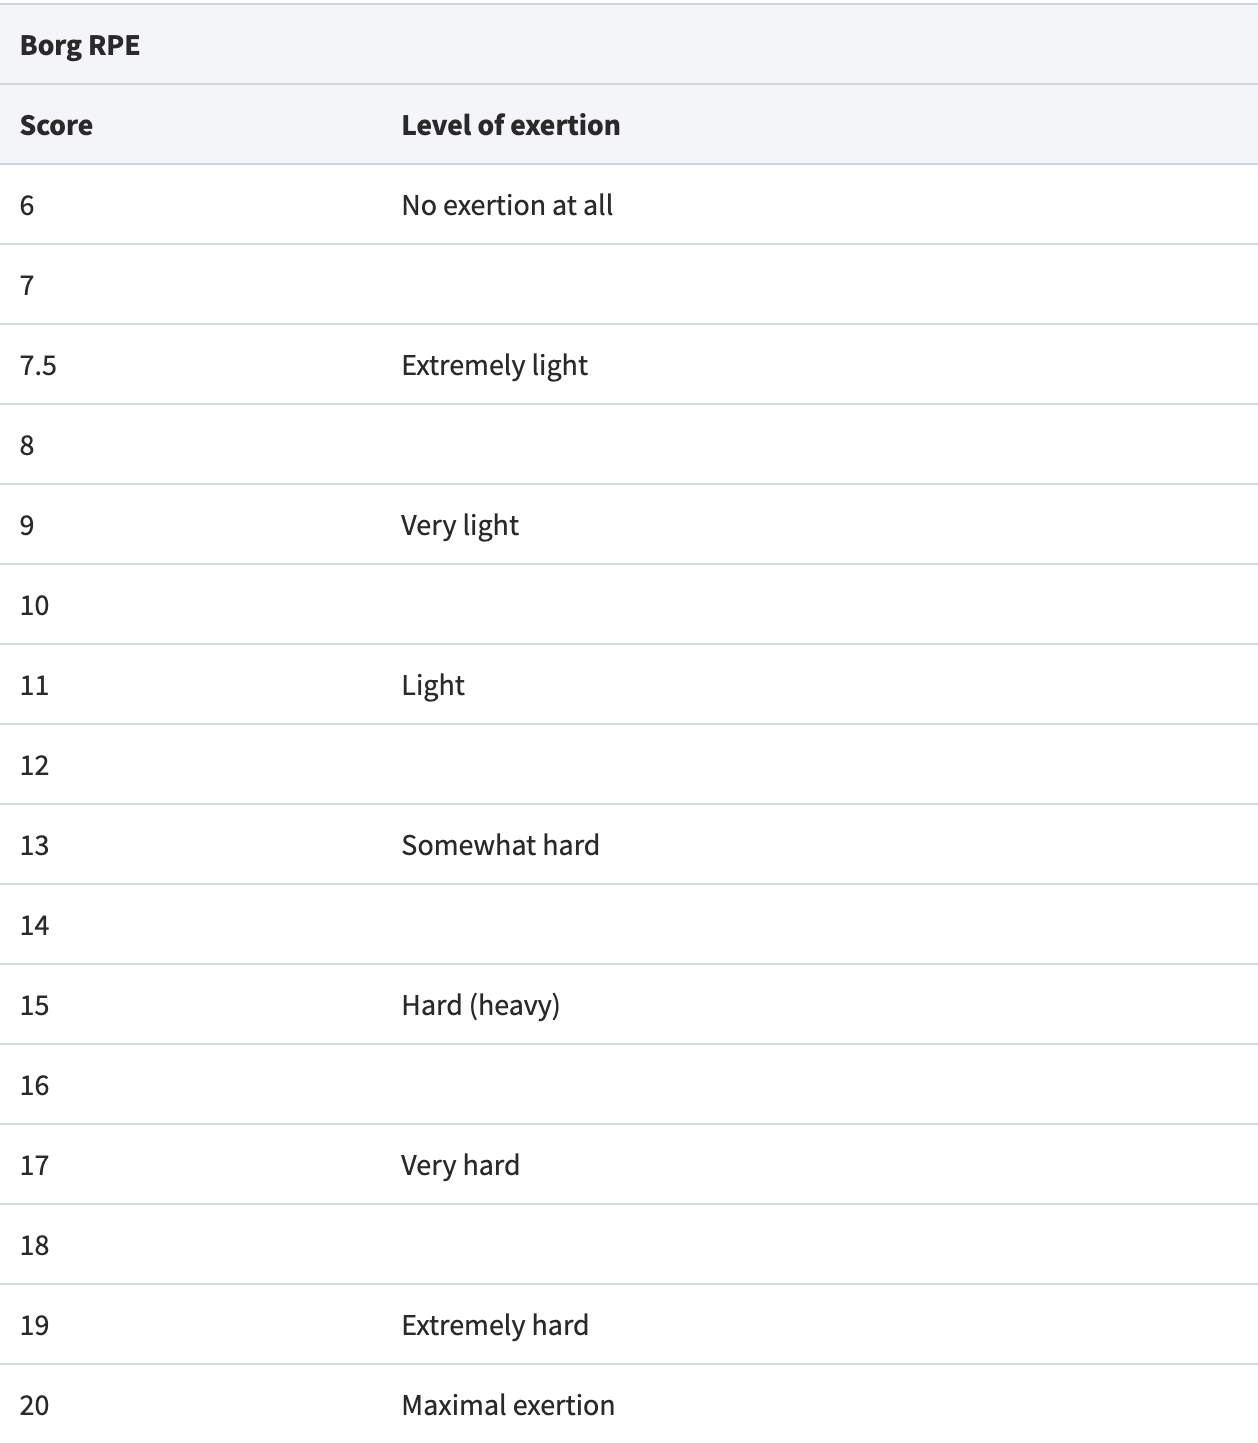
\includegraphics[width=\linewidth]{figures/borg20.png}
      \captionsetup{justification=centering}
      \caption[Borg 20]{The original Borg 6-20 RPE Scale \cite{Williams2017}} \label{fig:borg20}
  \end{minipage}\hfill
  \begin{minipage}[c]{0.4\linewidth}
      \centering
      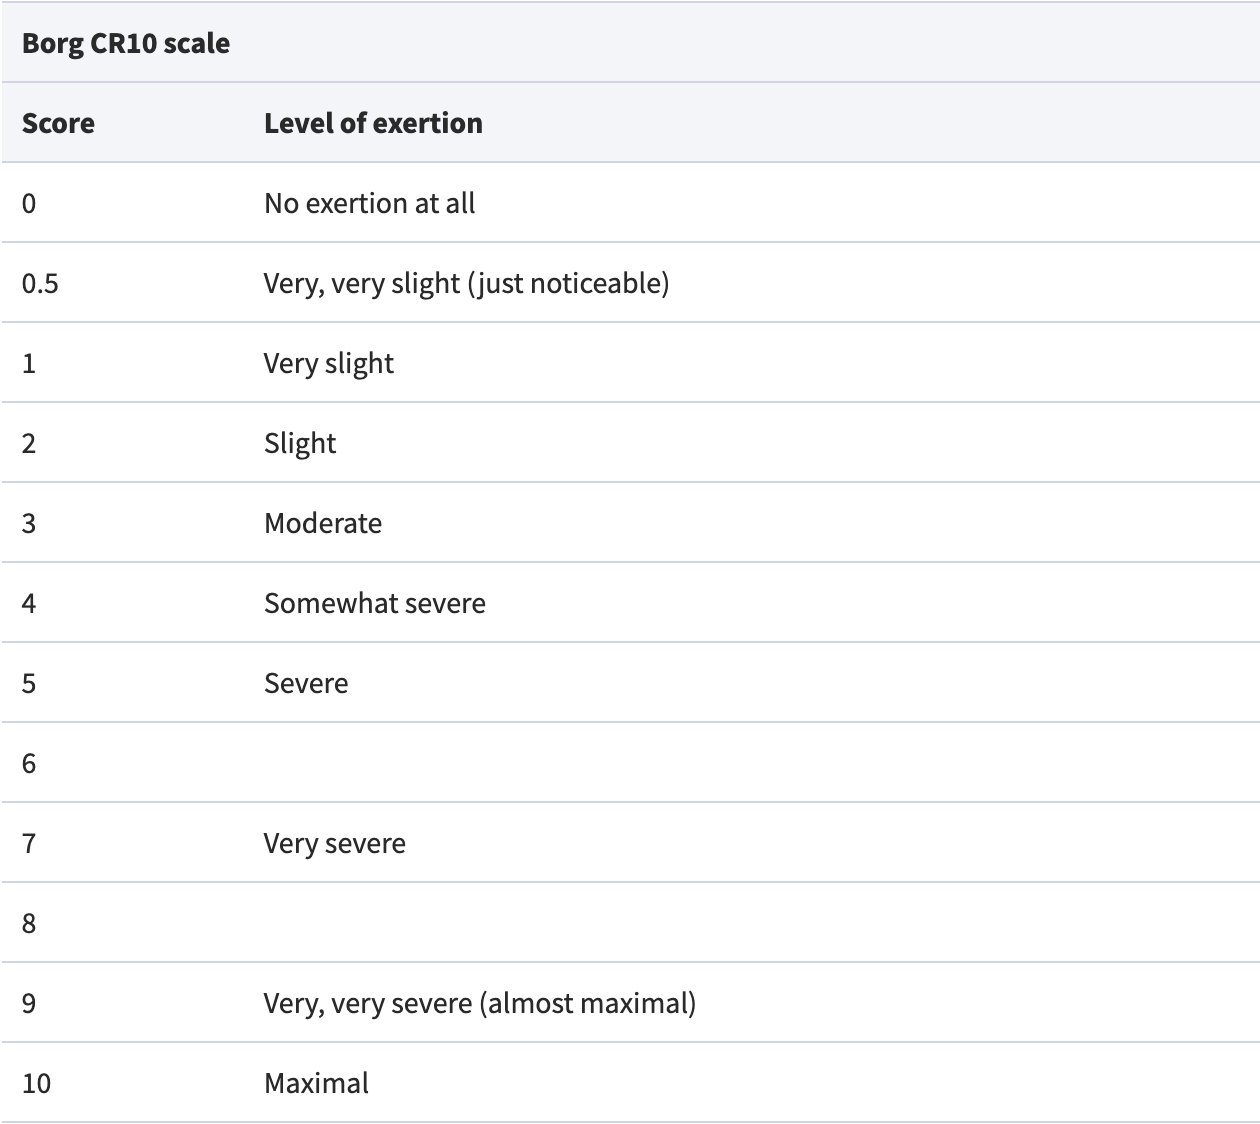
\includegraphics[width=\linewidth]{figures/borgc10.png}
      \captionsetup{justification=centering}
      \caption[Borg CR10]{The Borg Category-Ratio 10 RPE Scale \cite{Williams2017}}\label{fig:borgcr10}
  \end{minipage}
  \caption*{The two Borg RPE scales}
\end{figure}

\subsubsection{Training impulse (TRIMP)}
Training Impulse (TRIMP) is a method to calculate training load and is defined as  $\textnormal{TRIMP} = \textnormal{Training Volume} \times \textnormal{Training Intensity}$ \autocite{TRIMPmethod}. There are many methods to calculate TRIMP, using different metrics to calculate training volume and training intensity. For the purposes of this project volume will simply be minutes, and intensity will be average heart rate (bpm), as the simplest TRIMP method outlined. Other modifications may apply a weighting against a heart rate metric to normalise longer sessions completed at a lower heart rate -- considering the noted difference in heart rate responses to training in male and female athletes \autocite{Morton1990}, alternatively, load can be calculated by using the product of RPE and duration (ie. $\textnormal{RPE} \times \textnormal{Duration (minutes)}$).

\subsubsection{Acute chronic workload ratio (ACWR)}
Acute Chronic Workload Ratio (ACWR) can be used to monitor load in an athlete. It compares training load accumulated, in arbitrary units (AU), over the last seven days (acute workload) to the training load accumulated over the last twenty-eight days (chronic workload). The exact calculations used to determine acute and chronic workload depends on what type of ACWR model is selected. Additionally, the exact time periods considered for acute and chronic load can change depending on the application \cite{White2023}. Typically ACWR is used for injury management in team sports, but some articles have found it may not be effective for preventing injury as it is inaccurate way of approximating load \cite{Impellizzeri2020}. Training load estimation in rowing tends to be more objective given the objective internal load measurement of heart rate measured during a session. There is no clear consensus in literature about the effectiveness of using ACWR in injury prevention. As a relatively new concept, first published in 2016, more research into its efficacy and to provide validation needs to be completed \cite{Zouhal2021}. Regardless of its effectiveness in reducing injury, ACWR charts are easy to produce and provide easy feedback to rowers to see how training load can change week-to-week and ensuring load is not increased too quickly to begin to risk overtraining or injury.

\subsection{Impulse-Response Models} 
Impulse-response models are a group of models, built on the model initially introduced by \textcite{Bannister1976}. These models assume that a single exercise, or training session, produces two responses: fitness, or a positive performance response, and fatigue, or a negative performance response. A simplified version of this model is defined as 
\begin{equation}\label{eq:ffm}
  Performance = Fitness - Fatigue
\end{equation}
This simplified model is commonly called the Fitness-Fatigue impulse response model (FFM) and research since its initial introduction in 1975 has sought to refine how the $Fitness$ and $Fatigue$ components of this equation are defined.

\subsubsection{Banister fitness-fatigue model}
 In the FFM model originally introduced in 1975 \cite{Bannister1976}, and built upon by \textcite{Morton1990} in 1990, the functions for fitness and fatigue were defined, considering a cumulative training load and a decay factor for each response. This decay factor is different for both the fitness and fatigue responses, resulting in a longer decay period for fitness than fatigue, but also differs from person to person, offering a parameter to be tuned for each athlete. First, a session needs to be quantified. A session is defined as:
\begin{equation}\label{eq:ban_imp_base}
  w(t) = D (\Delta \textnormal{HR ratio})
\end{equation}
where
\begin{equation*}
  \Delta \textnormal{HR ratio} = \frac{\textnormal{HR}_\textnormal{exercise} - \textnormal{HR}_\textnormal{rest}}{\textnormal{HR}_\textnormal{max} - \textnormal{HR}_\textnormal{rest}}
\end{equation*}
\textcite{Morton1990} acknowledged the disproportionate influence longer sessions at a low heart rate could have on resulting sessions $w(t)$, in arbitrary units (AU), so introduced a weighting factor $Y$. They determined $Y = e^{bx}$, where $b$ is a pre-selected value determined for men and women, and $x = \Delta \textnormal{HR ratio}$. So each training session is calculated as:
\begin{equation}\label{eq:ban_impulse}
  w(t) = D (\Delta \textnormal{HR ratio})Y
\end{equation}
Next, Fitness, $g(t)$, and Fatigue, $h(t)$, can be calculated. These two functions are defined as
\begin{equation}\label{eq:ban_fit}
  g(t) = g(t - 1)e^\frac{-i}{\tau_1} + w(t)
\end{equation}
and
\begin{equation}\label{eq:ban_fat}
  h(t) = h(t - 1)e^\frac{-i}{\tau_2} + w(t)
\end{equation}
where each function states the fitness and fatigue at the end of the day $t$, $i$ is the number of days between the training session being added and the last training session, and $\tau_1$ and $\tau_2$ are the decay time constants for fitness and fatigue respectively. Finally, to model performance, two more constants are introduced: $k_1$ and $k_2$. These constants are weighting factors for fitness and fatigue, they have "no direct physiological interpretation" \cite{Morton1990} but can be used to adjust the model for athletes who recover more quickly to heavy training load or require more time to recover from sessions across a taper period. Finally, performance is modelled as
\begin{equation}\label{eq:ban_perf}
  p(t) = k_1g(t)-k_2h(t)
\end{equation}
The model was originally developed using a swimmer. When evaluated using linear regression for the athlete-specific parameters ($\tau_1$, $\tau_2$, $k_1$, and $k_2$), the model reasonably estimates the performance outcome of a swimmer with relative confidence. No $r^2$ value is provided for the swimming application in 1975 \cite{Bannister1976}. In the 1990 model from \textcite{Morton1990}, two of the researchers participated in a training and testing regimen and a "good degree of fit" was observed, with $r^2$ values of 0.71 and 0.96 calculated for a slightly trained and an untrained runner respectively, with the former being given a starting 1000 AU points given some preexisting running fitness. The impulse-response model, if trained appropriately can help guide the structure and timing of a taper period for each athlete \cite{Morton1990}.
Versions of this kind of impulse-response model are used in basic analysis across many consumer fitness apps today, such as Training Peaks and Strava.

\subsubsection{Limitations to the impulse-response model}
The Banister FFM simplifies human physiology quite effectively. However, in order to tune the parameters of the model, regular "criterion" testing needs to occur. These are maximal efforts done at regular intervals. During the testing of the \textcite{Morton1990} model refinements, both participants tested roughly once per week, something which is not feasible for high-level endurance athletes. This dependency on regular testing to tune parameters makes it particularly difficult to implement effectively as a holistic model for rowers. Furthermore, the use of data to adjust model parameters results in less data being available to model training behaviour.

The model only considers training load, specifically endurance training load, as an indicator for performance. Given the power dominance in rowing, a training block with seemingly less training load, as a result of more time and energy spent doing strength training, this can result in a bigger performance when tested next which may not be explained by changes in endurance training load. Additionally, the model does not consider other factors such as recovery and non-training strain an athlete might experience.

Finally, if the model is not constantly updated, it cannot predict future performances effectively. For the purposes of this project, a model would require an understanding of training behaviours in order to model the physiological response, predicting future performances. By modelling physiological response, suggestions can be made to improve certain energy system efficiency or effectiveness if needed. 

Impulse-response models are still widely used to model training and adaptation for athletes, their simplicity being a key factor for this. To more effectively model performances, without the need for constant testing, alternative models can and should be used. Impulse-response models can still be used in machine learning solutions, though, but as part of a larger ensemble approach \cite{Imbach2022}.

\subsection{Alternative Models}
There are models which employ more complicated mathematical approaches. This section will explore one of the most developed models, Performance Potential (PerPot), and explore artificial neural network approaches used by a number of researchers in recent years.

\subsubsection{Performance potential (PerPot)}
Performance Potential (PerPot) was first introduced by \textcite{perl2001} in 2001. It is a performance potential meta-model which models responses to training input through a flow model. PerPot approaches performance modelling similarly to the impulse-response approach, each training load has an antagonistic response, two contradicting effects: response potential and strain potential. These can be compared to the impulse-response fitness and fatigue responses, respectively. Strain and response potentials impact the performance potential with differing decay factors, like impulse-response models as well. There have been reports of PerPot being effective in modelling cycling training \cite{Churchill2014}. PerPot, unfortunately, suffers from one of the key issues with impulse-response modelling: repeated testing is needed to tune the model's parameters. Additionally, due to the nature of the decay factors for strain and response potentials, the super-compensation effect is not considered with the basic PerPot model \cite{Churchill2014}. 

\subsubsection{Artificial neural network (ANN) approaches}
Artificial neural networks (ANN) have been used to effectively model performance based on training data as early as 2000 by \textcite{Edelmannnusser2002} where (200m - Backstroke) swimming performances at the 2000 Olympic Games were predicted based entirely on training data. In building their model, \textcite{Edelmannnusser2002} considered the use of linear models like the impulse-response model, but commented that biological adaptations are inherently non-linear, and therefore set out to "demonstrate that the adaptive behaviour of an elite female swimmer can be modelled by means of the non-linear mathematical method of artificial neural networks". 

Machine learning techniques require vast quantities of data in order to be effective. \textcite{Edelmannnusser2002}, however, used a single athlete, collecting 95 weeks of training data and 19 competitive performances. This is quite a small training set for a machine learning application. With only 19 performances to compare a performance model to, the risk of overfitting is significant. \textcite{Edelmannnusser2002} completed three data analysis steps to generate a model. The first two steps involved determining the impact of a 2-week taper period and the impact of a 2-week intense period immediately before the taper (3-4 weeks before competition) for steps one and two respectively. The final step combined the first two steps to determine the influence of the four weeks leading into competition. The result of this neural network approach was quite successful and \textcite{Edelmannnusser2002} concluded that neural networks can be effectively used on small datasets to predict performances. 

\textcite{Churchill2014} sought to build on the success of using ANNs by \textcite{Edelmannnusser2002} to model performance outcomes, but targeting professional cycling performances. Churchill, however, struggled to collect data for peak performances due to the strategic nature of cycling. Churchill did develop techniques to smooth noise in small datasets using an ensemble approach, citing the larger the number of neural networks used, the better smoothing was applied to noise. Artificial neural networks have consistently shown promise in predicting performances in swimming and cycling, even addressing small dataset issues which are prevalent in machine learning applications. This project aspires to build on these successes and apply ANN and ensemble techniques to individual rowing training data to predict ergometer performances.
